\newpage
\section{Project Demo Scenario and Descriptors}

\begin{figure}[h]
\centering
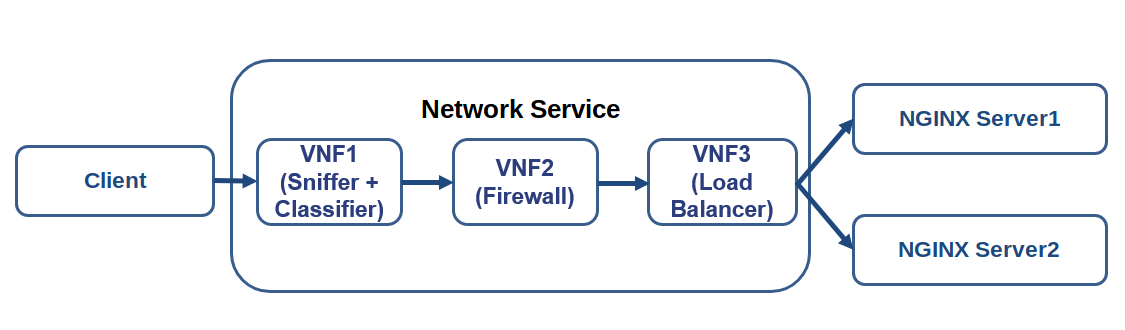
\includegraphics[width=1.0\linewidth]{figures/demoscenario}
\caption{Scenario architecture}
\label{fig:demoscenario}
\end{figure}


\subsection{Network Service Descriptor}
\begin{lstlisting}[language=yaml,caption=Demo NSD]
---
descriptor_version: '1.0'
vendor: pg-scramble
name: pg-scramble-demo
version: '0.1'
author: 'Arkajit Dhar'
description: 'The network service descriptor for the SCRAMBLE demo, comprising of a classifier, firewall and a loadbalancer'
network_functions:
    -
        vnf_id: vnf_classifier
        vnf_vendor: pg-scramble
        vnf_name: classifier-vnf
        vnf_version: '0.2'
    -
        vnf_id: vnf_firewall
        vnf_vendor: pg-scramble
        vnf_name: firewall-vnf
        vnf_version: '0.3'
    -
        vnf_id: vnf_loadbalancer
        vnf_vendor: pg-scramble
        vnf_name: loadbalancer-vnf
        vnf_version: '0.1'
connection_points:
    -
        id: mgmt
        interface: ipv4
        type: management
    -
        id: input
        interface: ipv4
        type: external
    -
        id: output
        interface: ipv4
        type: external
virtual_links:
    -
        id: mgmt
        connectivity_type: E-LAN
        connection_points_reference:
            - 'vnf_classifier:mgmt'
            - 'vnf_firewall:mgmt'
            - 'vnf_loadbalancer:mgmt'
            - mgmt
    -
        id: input-2-classifier
        connectivity_type: E-Line
        connection_points_reference:
            - input
            - 'vnf_classifier:input'
    -
        id: classifier-2-firewall
        connectivity_type: E-Line
        connection_points_reference:
            - 'vnf_classifier:output'
            - 'vnf_firewall:input'
    -
        id: firewall-2-loadbalancer
        connectivity_type: E-Line
        connection_points_reference:
            - 'vnf_firewall:output'
            - 'vnf_loadbalancer:input'
    -
        id: loadbalancer-2-output
        connectivity_type: E-Line
        connection_points_reference:
            - 'vnf_loadbalancer:output'
            - output
\end{lstlisting}

\subsection{VNF1}

\begin{lstlisting}[language=yaml,caption=Classifier VNFD]
---
descriptor_version: vnfd-schema-01
vendor: pg-scramble
name: classifier-vnf
version: '0.2'
author: 'Arkajit Dhar'
description: "A ubuntu sniffer-classifier image servers(2 ports:\ninput+output) in a single VNF"
virtual_deployment_units:
    -
        id: vdu01
        vm_image: sniffer-classifier-image
        vm_image_format: qcow2
        resource_requirements:
            cpu: {vcpus: 1}
            memory: {size: 1024, size_unit: MB}
            storage: {size: 5, size_unit: GB}
        connection_points:
            - {id: eth0, interface: ipv4, type: management}
            - {id: eth1, interface: ipv4, type: internal}
            - {id: eth2, interface: ipv4, type: internal}
virtual_links:
    -
        id: mgmt
        connectivity_type: E-LAN
        connection_points_reference:
            - 'vdu01:eth0'
            - mgmt
    -
        id: input
        connectivity_type: E-Line
        connection_points_reference:
            - 'vdu01:eth1'
            - input
    -
        id: output
        connectivity_type: E-Line
        connection_points_reference:
            - 'vdu01:eth2'
            - output
connection_points:
    -
        id: mgmt
        interface: ipv4
        type: management
    -
        id: input
        interface: ipv4
        type: external
    -
        id: output
        interface: ipv4
        type: external
\end{lstlisting}

\subsection{VNF2}

\begin{lstlisting}[language=yaml,caption=Firewall VNFD]
---
descriptor_version: vnfd-schema-01
vendor: pg-scramble
name: firewall-vnf
version: '0.3'
author: 'Arkajit Dhar'
description: "ubuntu base firewall with 2 ports:\ninput+output)"
virtual_deployment_units:
    -
        id: vdu01
        vm_image: firewall-image
        vm_image_format: qcow2
        resource_requirements:
            cpu: {vcpus: 1}
            memory: {size: 1024, size_unit: MB}
            storage: {size: 5, size_unit: GB}
        connection_points:
            - {id: eth0, interface: ipv4, type: management}
            - {id: eth1, interface: ipv4, type: internal}
            - {id: eth2, interface: ipv4, type: internal}
virtual_links:
    -
        id: mgmt
        connectivity_type: E-LAN
        connection_points_reference:
            - 'vdu01:eth0'
            - mgmt
    -
        id: input
        connectivity_type: E-Line
        connection_points_reference:
            - 'vdu01:eth1'
            - input
    -
        id: output
        connectivity_type: E-Line
        connection_points_reference:
            - 'vdu01:eth2'
            - output
connection_points:
    -
        id: mgmt
        interface: ipv4
        type: management
    -
        id: input
        interface: ipv4
        type: external
    -
        id: output
        interface: ipv4
        type: external
\end{lstlisting}

\subsection{VNF3}

\begin{lstlisting}[language=yaml,caption=Load balancer VNFD]
---
descriptor_version: vnfd-schema-01
vendor: pg-scramble
name: loadbalancer-vnf
version: '0.1'
author: 'Arkajit Dhar'
description: "A ubuntu image loadbalancer (2 ports:\ninput+output) in a single VNF"
virtual_deployment_units:
    -
        id: vdu01
        vm_image: loadbalancer-image
        vm_image_format: qcow2
        resource_requirements:
            cpu: {vcpus: 1}
            memory: {size: 1024, size_unit: MB}
            storage: {size: 5, size_unit: GB}
        connection_points:
            - {id: eth0, interface: ipv4, type: management}
            - {id: eth1, interface: ipv4, type: internal}
            - {id: eth2, interface: ipv4, type: internal}
virtual_links:
    -
        id: mgmt
        connectivity_type: E-LAN
        connection_points_reference:
            - 'vdu01:eth0'
            - mgmt
    -
        id: input
        connectivity_type: E-Line
        connection_points_reference:
            - 'vdu01:eth1'
            - input
    -
        id: output
        connectivity_type: E-Line
        connection_points_reference:
            - 'vdu01:eth2'
            - output
connection_points:
    -
        id: mgmt
        interface: ipv4
        type: management
    -
        id: input
        interface: ipv4
        type: external
    -
        id: output
        interface: ipv4
        type: external
\end{lstlisting}


